% !TEX root = saveliev_physics_general_course_1.tex
% !TEX TS-program = pdflatex
% !TEX encoding = UTF-8 Unicode





% check văn phong, định nghĩa, trau chuốt câu 
% check mis, error 57
% cross-check source code
% line 515, need more search for "whence"
% ask for using/translate words at line 22, 28, 57(extended bodies), 57($i$-th) (in queue)




\chapter{VẠN VẬT HẤP DẪN}\label{chap:6}

\section{Định luật vạn vật hấp dẫn}\label{sec:6_1}

Tất cả các vật thể trong tự nhiên đều tự hút lẫn nhau. Định luật mà lực hút này tuân theo được tìm ra/tuyên bố bởi Newton và được gọi là \textbf {Định luật vạn vật hấp dẫn}. Định luật này phát biểu như sau: \textit {lực mà hai chất điểm hút lẫn nhau có độ lớn tỉ lệ  thuận với (tích) khối lượng của chúng và tỉ lệ nghịch với bình phương khoảng cách giữa chúng}:
\begin{equation}\label{eq:6_1}
	F = G\frac{m_1m_2}{r^2}.
\end{equation}

\noindent
Ở đây $G$ là hằng số tỉ lệ được gọi là hằng số hấp dẫn. Lực hướng dọc theo đường thẳng đi qua/nối giữa các/hai hạt tương tác (\fig{6_1}).

\begin{figure}[!htb]
	\begin{minipage}[t]{0.5\linewidth}
		\begin{center}
			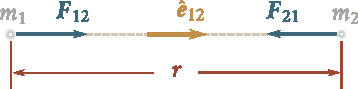
\includegraphics[scale=0.95]{figures/ch_06/fig_6_1.pdf}
			\caption[]{}
			\label{fig:6_1}
		\end{center}
	\end{minipage}
	\hspace{-0.05cm}
	\begin{minipage}[t]{0.5\linewidth}
		\begin{center}
			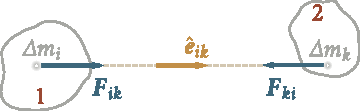
\includegraphics[scale=1]{figures/ch_06/fig_6_2.pdf}
			\caption[]{}
			\label{fig:6_2}
		\end{center}
	\end{minipage}
\end{figure}

Lực hấp dẫn của hạt thứ hai(2) hút/tác dụng lên hạt thứ nhất(1) có thể được viết/biểu diễn dưới dạng vector như sau
% The force with which the second particle attracts the first one can be written in the vector form as follows:
\begin{equation}\label{eq:6_2}
	\vec{F}_{12} = G\frac{m_1m_2}{r^2}\vecuni{12}.
\end{equation}

Ký hiệu $\vecuni{12}$ là viết tắt của một vector đơn vị hướng từ hạt đầu tiên đến hạt thứ hai(xem \fig{6_1}). Thay vector $\vecuni{21}$ cho vector $\vecuni{12}$ ở/trong \eqn{6_2}, ta nhận được lực $\vec{F}_{21}$ tác dụng lên hạt thứ hai.
% The symbol $\vecuni{12}$ stands for a unit vector directed from the first particle to the second one (see \fig{6_1}). Substituting the vector $\vecuni{21}$ for the vector $\vecuni{12}$ in \eqn{6_2}, we get the force $\vec{F}_{21}$ acting on the second particle.

Để tìm lực tương tác của các vật thể kéo dài, chúng phải được chia thành các khối lượng nguyên tố $\Delta m$, mỗi khối lượng có thể được giả định là một hạt chất điểm (\fig{6_2})). Theo \eqn{6_2}, khối lượng nguyên tố thứ $i$-th của vật thể $1$ bị hút bởi lực lượng $k$ -th khối lượng nguyên tố của vật thể $2$
% To find the force of interaction of extended bodies, they must be divided into elementary masses $\Delta m$, each of which can be assumed to be a point particle (\fig{6_2}). According to \eqn{6_2}, the $i$-th elementary mass of body $1$ is attracted to the $k$-th elementary mass of body $2$ with the force
\begin{equation}\label{eq:6_3}
	\vec{F}_{ik} = G\frac{\Delta m_i\Delta m_k}{r_{ik}^2}\vecuni{ik}
\end{equation}

\noindent
trong đó $r_{ik}$ là khoảng cách giữa các khối lượng nguyên tố.
% where $r_{ik}$ is the distance between the elementary masses.

Tính tổng của \eqn{6_3} trên tất cả các giá trị của chỉ số con $k$ tạo ra lực do vật $2$ tác dụng lên khối lượng nguyên tố $\Delta m_i$, thuộc phần thân $1$:
% Summation of \eqn{6_3} over all the values of the subscript $k$ gives the force exerted by body $2$ on the elementary mass $\Delta m_i$, belonging to body $1$:
\begin{equation}\label{eq:6_4}
	\vec{F}_{i2} = \sum_k G\frac{\Delta m_i\Delta m_k}{r_{ik}^2}\vecuni{ik}.
\end{equation}

\noindent
Cuối cùng, tổng của \eqn{6_4} trên tất cả các giá trị của chỉ số con $i$, \ie, tức là, tổng các lực tác dụng lên tất cả các khối lượng nguyên tố của vật thứ nhất cho lực do vật $2$ tác dụng lên vật $1$:
% Finally, summation of \eqn{6_4} over all the values of the subscript $i$, \ie, summation of the forces applied to all the elementary masses of the first body gives the force exerted by body $2$ on body $1$:
\begin{equation}\label{eq:6_5}
	\vec{F}_{12} = \sum_i \sum_k G\frac{\Delta m_i\Delta m_k}{r_{ik}^2}\vecuni{ik}.
\end{equation}

\noindent
Tính tổng được thực hiện trên tất cả các giá trị của các chỉ số phụ $i$ và $k$. Do đó, nếu phần thân $1$ được chia thành $N_1$ và phần thân $2$ thành $N_2$ khối lượng nguyên tố, thì tổng ~\eqref{eq:6_5} sẽ chứa $N_1N_2$ phần phụ.
% Summation is performed over all the values of the subscripts $i$ and $k$. Consequently, if body $1$ is divided into $N_1$, and body $2$ into $N_2$ elementary masses, then the sum~\eqref{eq:6_5} will contain $N_1N_2$ addends.

Trong thực tế, phép tính tổng theo \eqn {6_5} bao gồm tích phân và nói chung, là một vấn đề toán học rất phức tạp. Nếu các vật thể tương tác là đồng nhất và có hình dạng thông thường, các phép tính sẽ được đơn giản hóa rất nhiều. Đặc biệt, khi các vật thể tương tác là đồng nhất \footnote{Việc phân bố khối lượng trong giới hạn của mỗi quả cầu là đủ để có đối xứng trung tâm, \ie, nghĩa là mật độ chỉ là một hàm của khoảng cách từ tâm của hình cầu.} hình cầu, phép tính bằng \eqn{6_5} dẫn đến \eqn{6_2}, $m_1$ và $m_2$ bây giờ là khối lượng của các hình cầu, $r$ khoảng cách giữa các tâm của chúng và $\vecuni{12}$ một vector đơn vị hướng từ tâm của hình cầu thứ nhất đến tâm của hình cầu thứ hai. Do đó, các quả cầu tương tác giống như các hạt điểm có khối lượng bằng khối lượng của các quả cầu và nằm ở tâm của chúng.
% In practice, the summation according to \eqn{6_5} consists in integration and, generally speaking, is a very complicated mathematical problem. If the interacting bodies are homogeneous and have a regular shape, the calculations are greatly simplified. In particular, when the interacting bodies are homogeneous\footnote{It is sufficient for the distribution of the mass within the limits of each sphere to have central symmetry, \ie, for the density to be a function only of the	distance from the centre of the sphere.} spheres, calculation by \eqn{6_5} leads to \eqn{6_2}, $m_1$ and $m_2$ now being the masses of the spheres, $r$ the distance between their centres, and $\vecuni{12}$ a unit vector directed from the centre of the first sphere to that of the second one. The spheres thus interact like point particles of masses equal to those of the spheres and situated at their centres.

Nếu một trong các vật thể là một hình cầu đồng nhất có bán kính rất lớn (ví dụ: Trái đất), trong khi vật thể thứ hai có thể được coi là một hạt điểm, thì tương tác của chúng được mô tả bằng \eqn{6_2} trong đó $r$ là viết tắt của khoảng cách từ tâm quả cầu đến hạt (phát biểu này sẽ được chứng minh ở phần sau).
% If one of the bodies is a homogeneous sphere of a very great radius (for example, the Earth), while the second body can be considered as a point particle, then their interaction is described by \eqn{6_2} in which $r$ stands for the distance from the centre of the sphere to the particle (this statement will be proved in the following section).

Chiều của hằng số hấp dẫn theo \eqn{6_1} là
% The dimension of the gravitational constant in accordance with \eqn{6_1} is
\begin{equation*}
	[G] = \frac{[F][r^2]}{[m^2]} = \frac{(ML/T^2)L^2}{M^2} = L^3M^{-1}T^{-2}.
\end{equation*}

\noindent
Giá trị số của $G$ được xác định bằng cách đo lực mà hai vật có khối lượng đã biết hút nhau. Khó khăn lớn xuất hiện trong các phép đo như vậy vì lực hút là cực kỳ nhỏ đối với các vật thể có khối lượng có thể được đo trực tiếp. Ví dụ: hai vật thể có khối lượng \SI{100}{\kilo\gram} và cách nhau một mét tương tác với một lực có bậc \SI{e-6}{\newton}, \ie, tức là khoảng \SI{e-4}{\gf}.
% The numerical value of $G$ was determined by measuring the force with which two bodies of known mass attract each other. Great difficulties appear in such measurements because the forces of attraction are extremely small for bodies whose masses can be measured directly. For example, two bodies each having a mass of \SI{100}{\kilo\gram} and one metre apart interact with a force of the order of \SI{e-6}{\newton}, \ie, about \SI{e-4}{\gf}.

\begin{figure}[!htb]
	\begin{center}
		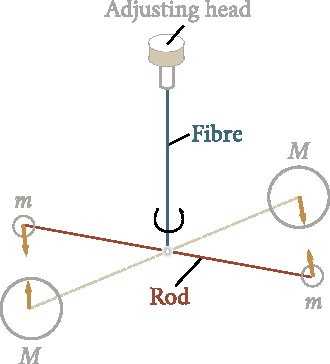
\includegraphics[scale=0.95]{figures/ch_06/fig_6_3.pdf}
		\caption[]{}
		\label{fig:6_3}
	\end{center}
\end{figure}

Nỗ lực thành công đầu tiên để xác định $G$ là phép đo của nó được thực hiện bởi Henry Cavendish (1731-1810) vào năm 1798. Ông đã sử dụng phương pháp cân bằng lực xoắn rất nhạy cảm (\fig{6_3}). Hai quả cầu chì $m$ (mỗi quả có khối lượng \SI{0.729}{\kilo\gram}) được gắn chặt vào hai đầu của một thanh nhẹ được đặt gần các quả cầu sắp xếp đối xứng $M$ (mỗi quả có khối lượng \SI{158}{\kilo\gram}). Thanh được treo trên một sợi xoắn đàn hồi. Độ xoắn của quả cầu sau đó đã được đo, và độ lớn của nó cho thấy lực hút giữa các quả cầu. Đầu trên của sợi quang được gắn chặt trong một đầu điều chỉnh có khả năng xoay để thay đổi khoảng cách giữa các quả cầu $m$ và $M$. Giá trị
% The first successful attempt to determine $G$ was its measurement carried out by Henry Cavendish (1731-1810) in 1798. He used the very sensitive torsion balance method (\fig{6_3}). Two lead spheres $m$ (each of mass \SI{0.729}{\kilo\gram}) fastened to the ends of a light rod were placed near symmetrically arranged spheres $M$ (each of mass \SI{158}{\kilo\gram}). The rod was suspended on an elastic torsion fibre. Twisting of the latter was measured, and its magnitude showed the force of attraction between the spheres. The top end of the fibre was fastened in an adjusting head whose turning made it possible to change the distance between the spheres $m$ and $M$. The value
\begin{equation*}
	G = \SI{6.670e-11}{\metre\cubed\per\kilo\gram\per\second\squared}\,\,(\text{or}\,\, \si{\newton\metre\squared\per\kilo\gram\squared})
\end{equation*}

\noindent
được coi là giá trị chính xác nhất trong số các giá trị được xác định theo các cách khác nhau.
% is considered to be the most accurate of all the values determined in different ways.

Nếu trong \eqn{6_1} chúng ta giả sử rằng $m_1$, $m_2$ và $r$ thống nhất bằng nhau, thì lực về số bằng $G$. Do đó, hai quả cầu đều có khối lượng \SI{1}{\kilo\gram} có tâm cách nhau \ SI {1} {\ mét} hút nhau bằng một lực \SI{6.670e-11}{\newton}.
% If in \eqn{6_1} we assume that $m_1$, $m_2$, and $r$ equal unity, then the force numerically equals $G$. Thus, two spheres each having a mass of \SI{1}{\kilo\gram} whose centres are \SI{1}{\metre} apart attract each other with a force of \SI{6.670e-11}{\newton}.

\section{Trường Hấp Dẫn}\label{sec:6_2}

% Gravitational interaction is carried out through a gravitational field. Every body changes the properties of the space surrounding it---it sets up a gravitational field in this space. The field manifests itself in that another body placed in it experiences a force. The ``intensity'' of a gravitational field can obviously be assessed according to the magnitude of the force acting at a given point on a body of unit mass. Accordingly, the quantity
Tương tác hấp dẫn được thực hiện thông qua trường hấp dẫn. Mọi vật thể đều thay đổi các đặc tính của không gian xung quanh nó --- nó thiết lập một trường hấp dẫn trong không gian này. Trường thể hiện ở chỗ một cơ thể khác được đặt trong nó chịu một lực. Rõ ràng có thể đánh giá `` cường độ '' của trường hấp dẫn theo độ lớn của lực tác dụng tại một điểm nhất định lên một vật có khối lượng đơn vị. Theo đó, lượng

\begin{equation}\label{eq:6_6}
	\vec{g}' = \frac{\vec{F}}{m}
\end{equation}

\noindent
% is called the \textbf{gravitational intensity}, or the \textbf{gravitational field vector}. In \eqn{6_6}, $\vec{F}$ is the gravitational force acting on a point particle of mass $m$ at a given point of the field.
được gọi là \textbf{cường độ hấp dẫn}, hoặc \textbf{vector trường hấp dẫn}. Trong  \eqn{6_6}, $\vec{F}$ là lực hấp dẫn tác dụng lên một hạt điểm có khối lượng $m$ tại một điểm nhất định của trường.

% The dimension of $\vec{g}'$ coincides with that of acceleration. The intensity of the gravitational field near the Earth's surface equals the acceleration of free fall $\vec{g}$ (with an accuracy up to the correction due to the Earth's rotation, see Sec.~\ref{sec:4_2}).
Chiều của  $\vec{g}'$trùng với chiều của gia tốc. Cường độ của trường hấp dẫn gần bề mặt Trái đất bằng với gia tốc rơi tự do $\vec{g}$ (với độ chính xác lên đến hiệu chỉnh do chuyển động quay của Trái đất, xem Phần~\ref{sec:4_2}).

% It is easy to conclude from \eqn{6_2} that the intensity of the field set up by a point particle of mass $m$ is
Từ \eqn{6_2} có thể dễ dàng kết luận rằng cường độ của trường do một hạt điểm có khối lượng $m$ thiết lập là
\begin{equation}\label{eq:6_7}
	\vec{g}' = -G\frac{m}{r^2}\vecuni{r}
\end{equation}

\noindent
% where $\vecuni{r}$ is the unit vector of the position vector drawn from the particle to the given point of the field, and $r$ is the magnitude of this position vector.
trong đó$\vecuni{r}$ là vector đơn vị của vector vị trí được vẽ từ hạt tới điểm đã cho của trường và $r$ là độ lớn của vector vị trí này.

% Assume that a gravitational field is produced by a point particle of mass $m$ fixed at the origin of coordinates. Hence, the following force will act on a particle of mass $m'$ at a point with the position vector $\vec{r}$:
Giả sử rằng một trường hấp dẫn được tạo ra bởi một hạt điểm có khối lượng $m$ cố định tại gốc tọa độ. Do đó, lực sau sẽ tác dụng lên một hạt có khối lượng $m'$ tại một điểm có vector vị trí $\vec{r}$:
\begin{equation}\label{eq:6_8}
	\vec{F} = \vec{g}'m' = -G\frac{mm'}{r^2}\vecuni{r}
\end{equation}

\noindent
% [compare with \eqn{3_120}]. We showed in Sec.~\ref{sec:3_13} that the potential energy of the particle $m'$ is determined in this case by the equation
[so sánh với \eqn{3_120}]. Chúng tôi đã chỉ ra trong Phần ~\ref{sec:3_13} rằng thế năng của hạt $m'$ được xác định trong trường hợp này bằng phương trình
\begin{equation}\label{eq:6_9}
	E_{\text{p}} = -G\frac{mm'}{r^2}
\end{equation}

\noindent
% (the potential energy is assumed to vanish when $r\to\infty$). Equation~\eqref{eq:6_9} can also be interpreted as the mutual potential energy of the point particles $m$ and $m'$.
(thế năng được cho là biến mất khi $r\to\infty$). Phương trình ~\eqref{eq:6_9} cũng có thể được hiểu là thế năng tương hỗ của các hạt điểm $m$ và $m'$.

% Inspection of \eqn{6_9} shows that to each point of the field produced by the particle $m$ there corresponds a definite value of the potential energy which the particle $m'$ has in this field. Consequently, the field can be characterized by the potential energy which a particle of mass $m'=1$ has at the given point. The quantity
Kiểm tra \eqn{6_9} cho thấy rằng tại mỗi điểm của trường được tạo ra bởi hạt $m$, tương ứng với một giá trị xác định của thế năng mà hạt $m'$ có trong trường này. Do đó, trường có thể được đặc trưng bởi thế năng mà một hạt có khối lượng $m'=1$ có tại điểm đã cho. Số lượng
\begin{equation}\label{eq:6_10}
	\varphi = \frac{E_{\text{p}}}{m'}
\end{equation}

\noindent
% is called the \textbf{potential of the gravitational field}. In this equation, $E_{\text{p}}$ is the potential energy which a point particle of mass $m'$ has at a given point of the field.
được gọi là \textbf{thế năng của trường hấp dẫn}. Trong phương trình này, $E_{\text{p}}$ là thế năng mà một hạt điểm có khối lượng $m'$ có tại một điểm nhất định của trường.

% Knowing the potential of a field, we can calculate the work done on the particle $m'$ by the forces of the field when moving it from position $1$ to position $2$. According to \eqn{3_30}, this work is
Biết thế năng của một trường, chúng ta có thể tính công thực hiện đối với hạt $m'$ bằng các lực của trường khi di chuyển nó từ vị trí $1$ đến vị trí $2$. Theo \eqn{3_30}, tác phẩm này là
\begin{equation}\label{eq:6_11}
	A_{12} = E_{\text{p},1} - E_{\text{p},2} = m'(\varphi_1 - \varphi_2).
\end{equation}

% According to Eqs.~\eqref{eq:6_6} and~\eqref{eq:6_10}, the force acting on the particle $m'$ is $\vec{F}=m'\vec{g}'$, and the potential energy of this particle is $E_{\text{p}}=m'\varphi$. By \eqn{3_31}, we have $\vec{F}=-\nabla E_{\text{p}}$, \ie, $m'\vec{g}'=-\nabla(m'\varphi)$. Putting the constant $m'$ outside the gradient sign and then cancelling this constant, we arrive at a relation between the intensity and potential of a gravitational field:
Theo các phương trình. ~\eqref{eq:6_6} và ~ \eqref{eq:6_10}, lực tác dụng lên hạt $m'$ là $\vec{F}=m'\vec{g}'$, và thế năng của hạt này là $E_{\text{p}}=m'\varphi$. Bởi\eqn{3_31}, chúng ta có $\vec{F}=-\nabla E_{\text{p}}$, \ie, $m'\vec{g}'=-\nabla(m'\varphi)$. Đặt hằng số $m'$ bên ngoài dấu gradient và sau đó hủy bỏ hằng số này, chúng ta đi đến mối quan hệ giữa cường độ và thế năng của trường hấp dẫn:
\begin{equation}\label{eq:6_12}
	\vec{g}' = -\nabla\varphi.
\end{equation}

\begin{figure}[!htb]
	\begin{center}
		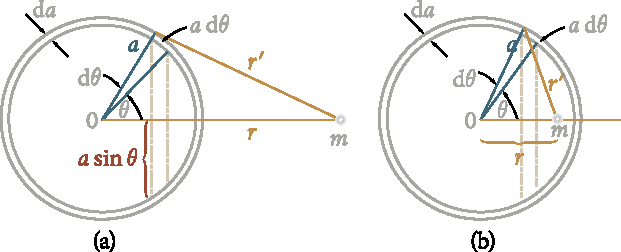
\includegraphics[scale=0.95]{figures/ch_06/fig_6_4.pdf}
		\caption[]{}
		\label{fig:6_4}
	\end{center}
\end{figure}

% Let us find an expression for the mutual potential energy of a homogeneous spherical layer and a point particle of mass $m$. We shall consider two cases corresponding to the particle being outside and inside the layer, and shall begin with the former one (\fig{6_4}a). Let us separate from the layer a ring whose edges correspond to the values of the angle $\theta$ and $\theta+\deriv{\theta}$. The radius of this ring is $a\sin\theta$, and its width is a $\deriv{\theta}$ (here $a$ is the radius of the layer). Hence, the area of the ring is determined by the expression $2\pi a^2\sin\theta\,\deriv{\theta}$. If the thickness of the layer is $\deriv{a}$ and its density is $\rho$, then the mass of the ring is $2\pi\rho a^2\,\deriv{a}\,\sin\theta\,\deriv{\theta}$. All the points of the ring are at the same distance $r'$ from $m$. Consequently, by \eqn{6_9}, the mutual potential energy of the ring and the mass $m$ is determined by the expression
Chúng ta hãy tìm biểu thức cho thế năng tương hỗ của một lớp hình cầu đồng chất và một hạt điểm có khối lượng $m$. Chúng ta sẽ xem xét hai trường hợp tương ứng với hạt ở bên ngoài và bên trong lớp, và sẽ bắt đầu với trường hợp trước (\fig{6_4}a). Chúng ta hãy tách khỏi lớp một vòng có các cạnh tương ứng với các giá trị của góc $\theta$ và $\theta+\deriv{\theta}$. Bán kính của vòng này là  $a\sin\theta$ và chiều rộng của nó là $\deriv{\theta}$ (ở đây $a$ là bán kính của lớp). Do đó, diện tích của vòng được xác định bởi biểu thức $2\pi a^2\sin\theta\,\deriv{\theta}$. Nếu độ dày của lớp là $\deriv{a}$ và mật độ của nó là $\rho$, thì khối lượng của vòng là $2\pi\rho a^2\,\deriv{a}\,\sin\theta\,\deriv{\theta}$. Tất cả các điểm của vòng đều ở cùng một khoảng cách $r'$ từ $m$. Do đó, theo \eqn{6_9}, thế năng tương hỗ của vòng và khối lượng $m$ được xác định bằng biểu thức
\begin{equation}\label{eq:6_13}
	\deriv{E_{\text{p}}} = -G\frac{2\pi\rho a^2\,\deriv{a}\,\sin\theta\,\deriv{\theta}\,m}{r'}.
\end{equation}

% To obtain the potential energy of the entire spherical layer and the mass $m$, we must integrate \eqn{6_13} with respect to the angle $\theta$ within the limits from $0$ to $\pi$. Here the variable $r'$ varies within the limits from $r-a$ to $r+a$, where $r$ is the distance from the centre of the layer $0$ to $m$. Equation~\eqref{eq:6_13} contains two related variables, namely, $a$ and $r'$. We must exclude one of these variables prior to integration. The latter is simplified if we exclude the variable $\theta$. We can obtain the relation between $\theta$ and $r'$ by using the theorem of cosines. Inspection of \fig{6_4} shows that
Để thu được thế năng của toàn bộ lớp hình cầu và khối lượng $ m $, chúng ta phải tích \eqn{6_13} với góc $\theta$ trong giới hạn từ $0$ đến $\pi$. Ở đây biến $r'$ thay đổi trong giới hạn từ $r-a$ đến $r+a$, trong đó $r$ là khoảng cách từ tâm của lớp $0$ đến $m$. Phương trình ~\eqref{eq:6_13} chứa hai biến có liên quan, đó là $a$ và $r'$. Chúng tôi phải loại trừ một trong các biến này trước khi tích hợp. Cái sau được đơn giản hóa nếu chúng ta loại trừ biến $\theta$. Chúng ta có thể thu được mối quan hệ giữa $\theta$ và $r'$ bằng cách sử dụng định lý cosin. Kiểm tra \fig{6_4} cho thấy rằng
\begin{equation*}
	r'^2 = a^2 + r^2 - 2ar\cos\theta.
\end{equation*}

\noindent
% Differentiation of this expression yields
Sự khác biệt của biểu thức này mang lại
\begin{equation*}
	2r'\,\deriv{r'} = 2ar\sin\theta\,\deriv{\theta}.
\end{equation*}

\noindent
% Hence, $\sin\theta\,\deriv{\theta}=(r'/ar)\,\deriv{r'}$. Making such a substitution in \eqn{6_13}, we get
Do đó, $\sin\theta\,\deriv{\theta}=(r'/ar)\,\deriv{r'}$. Thực hiện một sự thay thế như vậy trong \eqn{6_13}, chúng tôi nhận được
\begin{equation*}
	\deriv{E_{\text{p}}} = -G\frac{2\pi\rho a\,\deriv{a}\,m\,\deriv{r'}}{r}.
\end{equation*}

\noindent
% Integration with respect to $r'$ within the limits from $r_1'=r-a$ to $r_2'=r+a$ yields
Tích hợp đối với $r'$ trong giới hạn từ $r_1'=r-a$ thành $r_2'=r+a$ lợi nhuận
\begin{equation}\label{eq:6_14}
	\deriv{E_{\text{p,lay}}} = -G\frac{2\pi\rho a\,\deriv{a}\,m}{r} \int_{r-a}^{r+a} \deriv{r'} = -G\frac{4\pi\rho a^2\,\deriv{a}\,m}{r}.
\end{equation}

\noindent
% The expression $4\pi a^2\,\deriv{a}$ gives the volume of the layer, and $4\pi\rho a^2\,\deriv{a}$ its mass $\deriv{M}$. Thus, the mutual potential energy of the sphere layer and the mass $m$ is
Biểu thức $4\pi a^2\,\deriv{a}$ cho biết thể tích của lớp và $4\pi\rho a^2\,\deriv{a}$ khối lượng của nó $\deriv{M}$. Như vậy, thế năng lẫn nhau của lớp cầu và khối lượng $m$ là
\begin{equation}\label{eq:6_15}
	\deriv{E_{\text{p,lay}}} = -G\frac{\deriv{M}\,m}{r}
\end{equation}

\noindent
% where $r$ is the distance from the centre of the layer to $m$.
trong đó $r$ là khoảng cách từ tâm của lớp đến $m$.

% All our calculations remain the same for the case when the mass is inside the layer (see \fig{6_4}b). Only the integration limits in \eqn{6_14} will differ because $r'$ changes in this case from $r_1'=r-a$ to $r_2'=r+a$. Consequently,
Tất cả các tính toán của chúng tôi vẫn giữ nguyên đối với trường hợp khối lượng nằm bên trong lớp (xem \fig{6_4}b). Chỉ các giới hạn tích hợp trong \eqn{6_14} sẽ khác vì $r'$ thay đổi trong trường hợp này từ $r_1'=r-a$ thành $r_2'=r+a$. Do đó,
\begin{align}
	\deriv{E_{\text{p,lay}}'} &= -G\frac{2\pi\rho a\,\deriv{a}\,m}{r} \int_{a-r}^{a+r} \deriv{r'} = -G4\pi\rho a\,\deriv{a}\,m\nonumber\\
	& = -G \frac{4\pi\rho a^2\,\deriv{a}\,m}{a} = -G\frac{\deriv{M}\,m}{a}.\label{eq:6_16}
\end{align}

\noindent
% Hence, in this case the potential energy is the same for all $r'$s and equals the value obtained in \eqn{6_15} for $r=a$.
Do đó, trong trường hợp này, thế năng là như nhau đối với tất cả $r'$ s và bằng giá trị thu được trong \eqn{6_15} for $r=a$.

% Equation~\eqref{eq:6_15} can be interpreted as the potential energy of the particle $m$ in the field set up by a sphere layer of mass $\deriv{M}$. The derivative of this energy with respect to $r$ taken with the opposite sign equals the projection onto the direction $r$ of the force acting on the particle:
Phương trình~\eqref{eq: 6_15} có thể được hiểu là thế năng của hạt $m$ trong trường được thiết lập bởi một lớp hình cầu có khối lượng $\deriv{M}$. Đạo hàm của năng lượng này đối với $r$ lấy ngược dấu bằng hình chiếu lên phương $r$ của lực tác dụng lên hạt:
\begin{equation}\label{eq:6_17}
	\deriv{F_r} = -\diffpartial{E_{\text{p}}}{r} = -G\frac{\deriv{M}\,m}{r^2}.
\end{equation}

\noindent
% The minus sign indicates that the force is directed toward the diminishing of $r$, \ie, to the centre of the layer.
Dấu trừ chỉ ra rằng lực hướng tới sự giảm dần của $r$, tức là vào tâm của lớp.

% It follows from \eqn{6_17} that the sphere layer acts on the particle with the same force that would be exerted on it by a point particle of a mass equal to that of the layer and placed at the centre of the latter.
Theo \eqn{6_17}, lớp hình cầu tác dụng lên hạt với cùng một lực sẽ được tác dụng lên nó bởi một hạt điểm có khối lượng bằng với khối lượng của lớp và được đặt ở tâm của lớp sau.


% Equation~\eqref{eq:6_16} does not depend on the coordinates of a particle. Therefore, the gradient of this function vanishes for all $r'$s less than $a$. Thus, no force acts on a particle inside the layer. Every element of the layer naturally exerts a certain force on the particle, but the sum of the forces exerted by all the elements of the layer equals zero.
Phương trình ~\eqref{eq: 6_16} không phụ thuộc vào tọa độ của hạt. Do đó, gradient của hàm này biến mất đối với tất cả $r'$ s nhỏ hơn $a$. Do đó, không có lực nào tác động lên một hạt bên trong lớp. Mọi phần tử của lớp đều tác dụng một cách tự nhiên một lực nhất định lên hạt, nhưng tổng các lực do tất cả các phần tử của lớp tác dụng bằng không.


% Now let us consider a system consisting of a homogeneous sphere of mass $M$ and a point particle of mass $m$. Let us divide the sphere into layers of mass $\deriv{M}$. Each layer acts on the particle with a force determined by \eqn{6_17}. Summation of this expression over all the layers gives the force exerted on the particle by the sphere:
Bây giờ chúng ta hãy xem xét một hệ thống bao gồm một quả cầu đồng chất khối lượng $M$ và một hạt điểm khối lượng $m$. Chúng ta hãy chia khối cầu thành các lớp có khối lượng $\deriv{M}$. Mỗi lớp tác động lên hạt một lực được xác định bởi \eqn{6_17}. Tính tổng của biểu thức này trên tất cả các lớp cho lực tác dụng lên hạt bởi quả cầu:
\begin{equation}\label{eq:6_18}
	F_r = \int\deriv{F_r} = -\int G\frac{\deriv{M}\,m}{r^2} = -G\frac{Mm}{r^2}.
\end{equation}

\noindent
% The action of the sphere on the particle is equivalent to the action of a point particle of a mass equal to that of the sphere and placed at its centre (see the preceding section).
Tác dụng của quả cầu lên hạt tương đương với tác dụng của một hạt điểm có khối lượng bằng quả cầu và được đặt tại tâm của nó (xem phần trước).

% If we take a sphere with a spherical space inside, then no force will act on a particle in this space.
Nếu chúng ta lấy một quả cầu có không gian hình cầu bên trong, thì không có lực nào tác dụng lên một hạt trong không gian này.

% Summation of \eqn{6_15} over all the layers of a solid or a hollow sphere yields the mutual potential energy of a particle and a sphere:
Tính tổng \eqn{6_15} trên tất cả các lớp của một hình cầu đặc hoặc rỗng tạo ra thế năng tương hỗ của một hạt và một hình cầu:
\begin{equation}\label{eq:6_19}
	E_{\text{p}} = -G\frac{Mm}{r^2}.
\end{equation}

\noindent
% Here $M$ is the mass of the sphere, $m$ is the mass of the particle, and $r$ is the distance from the particle to the centre of the sphere.
Ở đây $M$ là khối lượng của quả cầu, $m$ là khối lượng của hạt và $r$ là khoảng cách từ hạt đến tâm của quả cầu.

% It follows from Eqs.~\eqref{eq:6_18} and~\eqref{eq:6_19} that the gravitational field produced by a homogeneous sphere is equivalent (outside the sphere) to the field produced by a point particle of the same mass at the centre of the sphere.
Theo phương trình~\eqref{eq:6_18} và~\eqref{eq:6_19} rằng trường hấp dẫn do một quả cầu đồng nhất tạo ra tương đương (bên ngoài quả cầu) với trường được tạo ra bởi một hạt điểm có cùng khối lượng ở tâm của mặt cầu.

% Let us consider two homogeneous spheres of masses $M_1$ and $M_2$. The second sphere experiences the same action on the part of the first one as would be exerted by a point particle of mass $M_1$ at the centre of the first sphere. According to Newton's third law, the corresponding force is equal in magnitude to the force that the second sphere would exert on the particle $M_1$. By \eqn{6_18}, the magnitude of this force is $GM_1M_2/r^2$. We have thus proved that homogeneous spheres interact like point particles at their centres.
Ta xét hai quả cầu đồng chất có khối lượng $M_1$ và $M_2$. Quả cầu thứ hai chịu tác dụng tương tự đối với phần của quả cầu thứ nhất khi được tác dụng bởi một hạt điểm có khối lượng $M_1$ tại tâm của quả cầu thứ nhất. Theo định luật thứ ba của Newton, lực tương ứng có độ lớn bằng lực mà quả cầu thứ hai tác dụng lên hạt $M_1$. Theo \eqn{6_18}, độ lớn của lực này là $GM_1M_2/r2$. Do đó, chúng tôi đã chứng minh rằng các quả cầu đồng nhất tương tác giống như các hạt điểm tại tâm của chúng.

\section{The Equivalence Principle}\label{sec:6_3}

% Mass comes up in two different laws---in Newton's second law and in the law of universal gravitation. In the former case, it characterizes the inertial properties of bodies, and in the latter their gravitational properties, \ie, the ability of bodies to attract one another. In this connection, the question arises whether we ought to distinguish the inertial mass $m_{\text{in}}$ and the gravitational mass $m_{\text{g}}$.
Khối lượng xuất hiện trong hai định luật khác nhau --- trong định luật thứ hai của Newton và trong định luật vạn vật hấp dẫn. Trong trường hợp trước, nó đặc trưng cho tính chất quán tính của các vật thể, và trong trường hợp sau là đặc tính hấp dẫn của chúng, \ie, tức là khả năng các vật thể hút nhau. Trong mối liên hệ này, câu hỏi đặt ra là liệu chúng ta có nên phân biệt khối lượng quán tính $m_{\text{in}}$ và khối lượng hấp dẫn $m_{\text{g}}$ hay không.

% This question can be answered only by experiments. Let us consider the free falling of bodies in a heliocentric reference frame. Any body near the Earth's surface experiences a force of attraction to the Earth that by \eqn{6_18} is
Câu hỏi này chỉ có thể được trả lời bằng các thí nghiệm. Chúng ta hãy coi sự rơi tự do của các vật thể trong hệ quy chiếu nhật tâm. Bất kỳ vật thể nào ở gần bề mặt Trái đất đều chịu một lực hút đối với Trái đất bằng \eqn{6_18} là
\begin{equation*}
	F = G\frac{m_{\text{g}} M_{\text{E}}}{R_{\text{E}}^2}
\end{equation*}

\noindent
% where $m_{\text{g}}$ is the gravitational mass of a given body, $M_{\text{E}}$ is the gravitational mass of the Earth, and $R_{\text{E}}$ is the radius of the Earth.
trong đó $m_{\text{g}}$ là trọng lượng hấp dẫn của một vật thể nhất định, $M_{\text{E}}$ là trọng lượng hấp dẫn của Trái đất và $R_{\text{E}}$ là bán kính của Trái đất.

% This force causes the body to acquire the acceleration $a$ (but not $g$, see Sec.~\ref{sec:4_2}) that must equal the force $F$ divided by the inertial mass of the body $m_{\text{in}}$:
Lực này làm cho vật có được gia tốc $a$ (nhưng không phải $g$, xem Phần ~\ref{sec:4_2}) phải bằng lực $F$ chia cho khối lượng quán tính của vật $m_{\text{in}}$:
\begin{equation}\label{eq:6_20}
	a = \frac{F}{m_{\text{in}}} = G\frac{M_{\text{E}}}{R_{\text{E}}^2}\frac{m_{\text{g}}}{m_{\text{in}}}.
\end{equation}

% Experiments show that the acceleration $a$ is the same for all bodies (it was shown in Sec.~\ref{sec:4_2} that the identical values of $a$ follow from the identical values of $g$). The factor $G(M_{\text{E}}/R_{\text{E}}^2)$ is also the same for all bodies. Consequently, the ratio $m_{\text{g}}/m_{\text{in}}$ is the same for all bodies too. All other experiments in which the difference between the inertial and the gravitational masses could manifest itself lead to a similar result.
Thử nghiệm cho thấy rằng gia tốc $a$ là như nhau đối với tất cả các phần tử (nó được hiển thị trong Phần ~\ref{sec:4_2} rằng các giá trị giống hệt nhau của $a$ tuân theo các giá trị giống nhau của $g$). Hệ số $G(M_{\text{E}}/R_{\text{E}}^2)$ cũng giống nhau đối với tất cả các phần tử. Do đó, tỷ lệ $m_{\text{g}}/m_{\text{in}}$ cũng giống nhau cho tất cả các nội dung. Tất cả các thí nghiệm khác trong đó sự khác biệt giữa khối lượng quán tính và hấp dẫn có thể dẫn đến một kết quả tương tự.

% We shall describe the experiment of R. E\"{o}tv\"{o}s, which he began in 1887 and continued over 25 years, as an example of such experiments. E\"{o}tv\"{o}s proceeded from the circumstance that a body at rest near the Earth's surface, apart from the reaction of its support, experiences the gravitational force $\vec{F}_{\text{g}}$ directed toward the Earth's centre and also the centrifugal force of inertia $\vec{F}_{\text{cf}}$ directed perpendicularly to the Earth's axis of rotation (\fig{6_5}---this figure is not drawn to scale---the magnitude of the centrifugal force is two orders smaller than that of the gravitational force, see Sec.~\ref{sec:4_2}). The gravitational force is proportional to the gravitational mass of a body $m_{\text{g}}$:
Chúng tôi sẽ mô tả thí nghiệm của R. E\"{o}tv\"{o}s, mà ông đã bắt đầu vào năm 1887 và tiếp tục trong 25 năm, như một ví dụ về các thí nghiệm như vậy. E\"{o}tv\"{o}s được tiến hành trong trường hợp một vật thể ở yên gần bề mặt Trái đất, ngoài phản ứng của lực hỗ trợ của nó, còn chịu lực hấp dẫn $\vec{F}_{\text{g}}$ hướng về tâm Trái đất và cũng là lực ly tâm của quán tính $\vec{F}_{\text{cf}}$ hướng vuông góc với trục quay của Trái đất (\fig{6_5} --- hình này không được vẽ theo tỷ lệ --- độ lớn của lực ly tâm nhỏ hơn hai bậc so với lực hấp dẫn, xem Phần ~\ref{sec:4_2}). Lực hấp dẫn tỷ lệ với trọng lượng của vật thể $m_{\text{g}}$:
\begin{equation*}
	\vec{F}_{\text{g}} = m_{\text{g}}\vec{g}'
\end{equation*}

\noindent
% ($\vec{g}'$ is the gravitational intensity). The centrifugal force of inertia is proportional to the inertial mass $m_{\text{in}}$. According to \eqn{4_7}, its magnitude is determined by the expression
(($\vec{g}'$ là cường độ trọng trường). Lực quán tính ly tâm tỷ lệ với khối lượng quán tính $m_{\text{in}}$. Theo \eqn{4_7}, độ lớn của nó được xác định bởi biểu thức
\begin{equation*}
	F_{\text{cf}} = m_{\text{in}}\omega^2R_{\text{E}}\cos\varphi
\end{equation*}

\noindent
% where $\varphi$ is the latitude of the locality. It follows from \fig{6_5} that the magnitude of the vertical component of the centrifugal force of inertia is
trong đó $\varphi$ là vĩ độ của địa phương. Theo từ \fig{6_5} thì độ lớn của thành phần thẳng đứng của lực quán tính ly tâm là
\begin{equation*}
	F_{\text{vert}} = F_{\text{cf}}\cos\varphi =  m_{\text{in}}\omega^2R_{\text{E}}\cos^2\varphi = Am_{\text{in}}.
\end{equation*}

\noindent
% We have introduced the symbol $A=\omega^2R_{\text{E}}\cos^2\varphi$. E\"{o}tv\"{o}s ran his experiment at the latitude of $\varphi=\SI{45}{\degree}$. In this case the coefficient $A$ is about one-hundredth of $g'$.
Chúng tôi đã giới thiệu ký hiệu $A=\omega^2R_{\text{E}}\cos^2\varphi$. E\"{o}tv\"{o}s đã chạy thử nghiệm của mình ở vĩ độ $\varphi=\SI{45}{\degree}$. Trong trường hợp này, hệ số $A$ bằng khoảng một phần trăm của $g'$.

\begin{figure}[!htb]
	\begin{minipage}[t]{0.5\linewidth}
		\begin{center}
			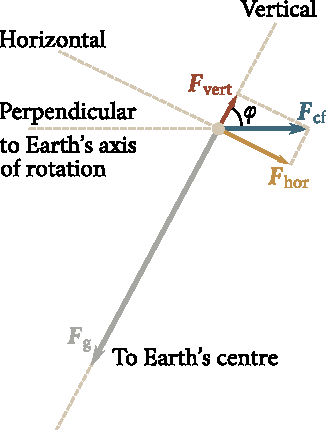
\includegraphics[scale=0.9]{figures/ch_06/fig_6_5.pdf}
			\caption[]{}
			\label{fig:6_5}
		\end{center}
	\end{minipage}
	\hspace{-0.05cm}
	\begin{minipage}[t]{0.5\linewidth}
		\begin{center}
			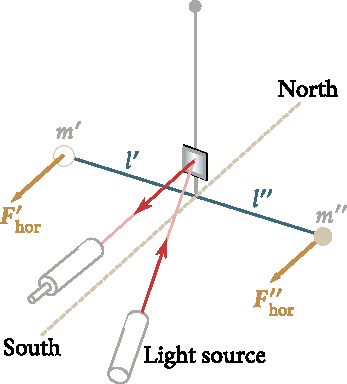
\includegraphics[scale=0.9]{figures/ch_06/fig_6_6.pdf}
			\caption[]{}
			\label{fig:6_6}
		\end{center}
	\end{minipage}
\end{figure}

% The magnitude of the horizontal component of the force $F_{\text{cf}}$ is
Độ lớn của thành phần nằm ngang của lực $F_{\text{cf}}$ là
\begin{equation*}
	F_{\text{hor}} = F_{\text{cf}}\sin\varphi =  m_{\text{in}}\omega^2R_{\text{E}}\cos\varphi\sin\varphi = Bm_{\text{in}}
\end{equation*}

\noindent
% where $B=\omega^2R_{\text{E}}\cos\varphi\sin\varphi$ (for $\varphi=\SI{45}{\degree}$, the values of the coefficients A and B coincide).
trong đó $B=\omega^2R_{\text{E}}\cos\varphi\sin\varphi$ (cho $\varphi=\SI{45}{\degree}$, giá trị của các hệ số A và B trùng nhau ).

% E\"{o}tv\"{o}s suspended a rod with bodies fastened to its ends on an elastic thread (\fig{6_6}). The bodies were of different materials, but their masses were as equal as possible. A mirror was attached to the bottom part of the thread. The beam from the light source reflected from the mirror struck the cross hairs of a telescope. The arms $l'$ and $l''$ were selected so that the rod was in equilibrium in the vertical plane. The condition for this equilibrium is as follows:
E\"{o}tv\"{o}s được treo một thanh có thân được buộc chặt vào các đầu của nó trên một sợi đàn hồi (\fig{6_6}). Các cơ thể được làm bằng các vật liệu khác nhau, nhưng khối lượng của chúng càng bằng nhau càng tốt. Một chiếc gương được gắn vào phần dưới cùng của sợi chỉ. Chùm sáng từ nguồn sáng phản xạ từ gương chiếu vào các sợi lông chéo của kính thiên văn. Các cánh tay $l'$ và $l''$ được chọn sao cho thanh ở trạng thái cân bằng trong mặt phẳng thẳng đứng. Điều kiện cho trạng thái cân bằng này như sau:
\begin{equation}\label{eq:6_21}
	(m_{\text{g}}'g' - m_{\text{in}}'A)l' = (m_{\text{g}}''g' - m_{\text{in}}''A)l''.
\end{equation}

\noindent
% The instrument was arranged with the rod perpendicular to the plane of the meridian (see \fig{6_6}). In this case, the horizontal components of the centrifugal force of inertia set up a twisting moment equal to
Dụng cụ được bố trí với thanh vuông góc với mặt phẳng của kinh tuyến (xem \fig{6_6}). Trong trường hợp này, các thành phần nằm ngang của lực quán tính ly tâm thiết lập một mômen xoắn bằng
\begin{equation}\label{eq:6_22}
	M_{\text{t}} = m_{\text{in}}'Bl' - m_{\text{in}}''Bl''.
\end{equation}

\noindent
% Eliminating the arm $l''$ from Eqs.~\eqref{eq:6_21} and~\eqref{eq:6_22}, we can arrive at the following equation after simple transformations:
Loại bỏ nhánh $l:$ khỏi phương trình ~\eqref{eq:6_21} và~\eqref{eq:6_22}, chúng ta có thể đi đến phương trình sau sau các phép biến đổi đơn giản:
\begin{equation*}
	M_{\text{t}} = m_{\text{in}}'Bl' \left[1 - \frac{(m_{\text{g}}'/m_{\text{in}}') g' - A}{(m_{\text{g}}''/m_{\text{in}}'') g' - A} \right].
\end{equation*}

\noindent
% It can be seen from this equation that when the ratio of the gravitational and inertia masses is the same for both bodies, the moment twisting the thread must vanish. If the ratio $m_{\text{g}}/m_{\text{in}}$ for the first and second bodies is not the same, the twisting moment differs from zero. In this case when the entire instrument is turned through \SI{180}{\degree}, the twisting moment would reverse its sign and the light spot would move from the cross hairs of the telescope (\fig{6_7}). E\"{o}tv\"{o}s compared eight different bodies (including a wooden one) with a platinum body taken as the standard and discovered no twisting of the thread. This gave him the grounds to state that the ratio $m_{\text{g}}/m_{\text{in}}$ for these bodies is identical with an accuracy of \num{e-8}.
Từ phương trình này có thể thấy rằng khi tỉ số giữa khối lượng hấp dẫn và quán tính đối với cả hai vật là như nhau thì mômen xoắn sợi chỉ phải biến mất. Nếu tỷ lệ $m_{\text{g}}/m_{\text{in}}$ cho phần thân thứ nhất và thứ hai không giống nhau, thì mômen xoắn khác 0. Trong trường hợp này khi toàn bộ dụng cụ được quay qua \SI{180}{\degree}, mômen xoắn sẽ đảo ngược dấu hiệu của nó và điểm sáng sẽ di chuyển từ các sợi chéo của kính thiên văn (\fig{6_7}). E\"{o}tv\"{o}s đã so sánh tám phần thân khác nhau (bao gồm cả phần thân bằng gỗ) với phần thân bằng bạch kim được lấy làm tiêu chuẩn và phát hiện ra không có sợi chỉ nào bị xoắn. Điều này giúp anh ta có cơ sở để tuyên bố rằng tỷ lệ $m_{\text{g}}/m_{\text{in}}$ cho các phần này là giống hệt nhau với độ chính xác là \num{e-8}.
\begin{figure}[!htb]
	\begin{center}
		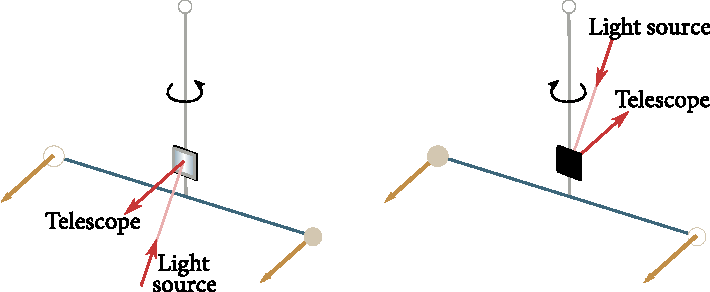
\includegraphics[scale=0.95]{figures/ch_06/fig_6_7.pdf}
		\caption[]{}
		\label{fig:6_7}
	\end{center}
\end{figure}

% In 1961-1964, R. Dicke improved E\"{o}tv\"{o}s's method. He used the Sun's gravitational field and the centrifugal force of inertia due to the Earth's orbital motion for producing the twisting moment. As a result of his measurements, he arrived at the conclusion that the ratio $m_{\text{g}}/m_{\text{in}}$ is the same for the studied bodies with an accuracy of \num{e-11}. Finally, in 1971, V. Braginsky and V. Panov obtained the constancy of the ratio with an accuracy up to \num{e-12}.
Năm 1961-1964, R. Dicke cải tiến phương pháp của E\"{o}tv\"{o}s. Ông đã sử dụng trường hấp dẫn của Mặt trời và lực quán tính ly tâm do quỹ đạo chuyển động của Trái đất để tạo ra mômen xoắn. Kết quả của các phép đo của mình, ông đã đi đến kết luận rằng tỷ lệ $m_{\text{g}}/m_{\text{in}}$ là như nhau đối với các cơ thể được nghiên cứu với độ chính xác là \num{e- 11}. Cuối cùng, vào năm 1971, V. Braginsky và V. Panov đã thu được hằng số của tỷ lệ với độ chính xác lên tới \num{e-12}.
% Thus, all the experimental facts indicate that the inertial and gravitational masses of all bodies are strictly proportional to each other. This signifies that these masses become identical when the units are selected properly. This is why physicists simply speak of mass. Albert Einstein based his general theory of relativity on the gravitational and inertial masses being identical.
Do đó, tất cả các dữ kiện thực nghiệm chỉ ra rằng khối lượng quán tính và trọng trường của tất cả các vật thể đều tỷ lệ thuận với nhau. Điều này cho thấy rằng các khối lượng này trở nên giống hệt nhau khi các đơn vị được chọn đúng cách. Đây là lý do tại sao các nhà vật lý chỉ đơn giản nói về khối lượng. Albert Einstein dựa trên lý thuyết tương đối rộng của mình dựa trên khối lượng hấp dẫn và quán tính là giống hệt nhau.

% We have already noted in Sec.~\ref{sec:4_1} that the forces of inertia are similar to gravitational forces---both are proportional to the mass of the body which they are acting on. We have indicated there that if we are in a closed cab, no experiments will help us to establish what the action of the force $m\vec{g}$ is due to---whether it is due to the cab moving with the acceleration $-\vec{g}$, or to the fact that the stationary cab is near the Earth's surface. This statement forms the content of the so-called \textbf{equivalence principle}.
Chúng ta đã lưu ý trong Sec. ~\ref{sec:4_1} rằng lực quán tính tương tự như lực hấp dẫn --- cả hai đều tỷ lệ với khối lượng của vật thể mà chúng đang tác động lên. Chúng tôi đã chỉ ra ở đó rằng nếu chúng tôi đang ở trong một chiếc taxi đã đóng cửa, không có thí nghiệm nào giúp chúng tôi xác định tác dụng của lực $m\vec{g}$ là do --- cho dù đó là do chiếc taxi chuyển động với gia tốc $-\vec{g}$, hoặc thực tế là chiếc taxi đứng yên gần bề mặt Trái đất. Câu lệnh này hình thành nội dung của cái gọi là \textbf{nguyên tắc tương đương}.

% The identical nature of inertial and gravitational masses is the result of the equivalence of forces of inertia and gravitational forces.
Bản chất giống hệt nhau của các khối lượng quán tính và hấp dẫn là kết quả của sự tương đương của lực quán tính và lực hấp dẫn.

% It must be noted that from the very beginning we assumed in \eqn{6_1} that the mass coincides with the inertial mass of bodies, and we therefore determined the numerical value of $G$ assuming that $m_{\text{g}}/m_{\text{in}}$. We can thus write \eqn{6_20} in the form
Cần lưu ý rằng ngay từ đầu, chúng tôi đã giả định trong \eqn{6_1} rằng khối lượng trùng với khối lượng quán tính của các vật thể và do đó chúng tôi xác định giá trị số của $G$ với giả định rằng $m_{\text{g}}/m_{\text{in}}$. Do đó, chúng tôi có thể viết \eqn{6_20} trong biểu mẫu
\begin{equation}\label{eq:6_23}
	a = G\frac{M_{\text{E}}}{R_{\text{E}}^2}.
\end{equation}

\noindent
% Equation~\eqref{eq:6_23} permits us to determine the mass of the Earth $M_{\text{E}}$. Use of the measured values of $a$, $R_{\text{E}}$ and $G$ in it gives the value of \SI{5.98e24}{\kilo\gram} for the Earth's mass.
Phương trình ~\eqref{eq:6_23} cho phép chúng tôi xác định khối lượng của Trái đất $M_{\text{E}}$. Việc sử dụng các giá trị đo được của $a$, $R_{\text{E}}$ và $G$ trong đó cho giá trị \SI{5.98e24}{\kilo\gram} cho khối lượng Trái đất.

% Further, knowing the radius of the Earth's orbit $R_{\text{orb}}$ and the time $T$ of one complete revolution of the Earth about the Sun, we can find the Sun's mass $M_{\text{S}}$. The Earth's acceleration equal to $\omega^2R_{\text{orb}}$ (the angular velocity $\omega=2\pi/T$) is due to the force with which the Sun attracts the Earth. Hence,
Hơn nữa, khi biết bán kính của quỹ đạo Trái đất $R_{\text{orb}}$ và thời gian $T$ của một vòng quay hoàn toàn của Trái đất về Mặt trời, chúng ta có thể tìm thấy khối lượng của Mặt trời $M_{\text{S}}$. Gia tốc của Trái đất bằng $\omega^2R_{\text{orb}}$ (vận tốc góc $\omega=2\pi/T$) là do lực mà Mặt trời hút Trái đất. Kể từ đây,
\begin{equation*}
	M_{\text{E}}\omega^2R_{\text{orb}} = G\frac{M_{\text{E}}M_{\text{S}}}{R_{\text{orb}}^2}
\end{equation*}

\noindent
% whence we can calculate the Sun's mass.
từ đó chúng ta có thể tính được khối lượng của Mặt trời.

% The masses of other celestial bodies were determined in a similar way.
Khối lượng của các thiên thể khác cũng được xác định theo cách tương tự.

\section{Vận tốc quỹ đạo và vận tốc thoát}\label{sec:6_4}

% To travel about the Earth in a circular orbit with a radius differing only slightly from the Earth's radius $R_{\text{E}}$, a body must have a definite velocity $v_1$. Its value can be found from the condition of equality of the product of the mass of the body and its acceleration to the force of gravity acting on the body:
Để đi quanh Trái đất theo quỹ đạo tròn có bán kính chỉ khác một chút so với bán kính Trái đất $R_ {\text {E}}$, vật thể phải có vận tốc xác định $v_1$. Giá trị của nó có thể được tìm thấy từ điều kiện bằng nhau của tích của khối lượng của vật thể và gia tốc của nó đối với lực hấp dẫn tác dụng lên vật thể:
\begin{equation*}
	m\frac{m_1^2}{R_{\text{E}}} = mg.
\end{equation*}

\noindent
% Hence,
Từ đây,
\begin{equation}\label{eq:6_24}
	v_1 = (gR_{\text{E}})^{1/2}.
\end{equation}

% Consequently, for a body to become a satellite of the Earth, it must be given the velocity $v_1$ called the \textbf{tangential} or \textbf{orbital velocity} ($v_1$ is also sometimes called the \textbf{first cosmic velocity}). Introduction of the values of $g$ and $R_{\text{E}}$ gives the following value for the orbital velocity:
Do đó, để một vật thể trở thành vệ tinh của Trái đất, nó phải có vận tốc $v_1$ được gọi là \textbf{tiếp tuyến} hoặc \textbf{vận tốc quỹ đạo} ($v_1$ đôi khi còn được gọi là \textbf{vũ trụ vận tốc cấp một}). Sự thay thế cho các giá trị của $g$ và $R _{\text{E}}$ đưa ra giá trị sau cho vận tốc quỹ đạo:
\begin{equation*}
	v_1 = (gR_{\text{E}})^{1/2} = (9.8 \times 6.4 \times 10^6)^{1/2} \approx \SI{8e3}{\metre\per\second} = \SI{8}{\kilo\metre\per\second}.
\end{equation*}

% A body having the velocity $v_1$ will not fall onto the Earth. This velocity, however, is not sufficient for the body to leave the sphere of the Earth's attraction, \ie, to travel away from the Earth over a distance such that its attraction to the Earth stops playing a significant part. The velocity $v_2$ required for this purpose is called the \textbf{escape velocity} (the \textbf{second cosmic velocity}).
Vật thể có vận tốc $v_1$ sẽ không rơi xuống Trái đất. Tuy nhiên, vận tốc này không đủ để vật thể rời thể tích cầu chịu lực hút của Trái đất, tức là di chuyển ra khỏi Trái đất một khoảng cách sao cho lực hút của nó đối với Trái đất ngưng đóng một vai trò đáng kể. Vận tốc $v_2$ cần thiết cho mục đích này được gọi là \textbf{vận tốc thoát} (\textbf{vận tốc vũ trụ cấp hai}).

% To find the escape velocity, we must calculate the work that must be done against the forces of the Earth's attraction for moving a body from the Earth's surface to infinity. When a body moves away, the forces of the Earth's attraction do the following work on it:
Để tìm vận tốc thoát, chúng ta phải tính toán công việc phải thực hiện để chống lại lực hút của Trái đất đối với việc di chuyển một vật thể từ bề mặt Trái đất đến vô cùng. Khi một vật chuyển động ra xa, lực hút của Trái đất tác dụng lên nó:
\begin{equation*}
	A' = E_{\text{p,init}} - E_{\text{p,fin}}.
\end{equation*}

\noindent
% According to \eqn{6_19}, the initial potential energy is
Theo \eqn{6_19}, thế năng ban đầu là
\begin{equation*}
	E_{\text{p,init}} = -G\frac{M_{\text{E}}m}{R_{\text{E}}}.
\end{equation*}

\noindent
% and the final potential energy is zero. Thus,
và thế năng cuối cùng bằng không. Vì vậy,
\begin{equation*}
	A' = -G\frac{M_{\text{E}}m}{R_{\text{E}}}.
\end{equation*}

\noindent
% The work $A$ that must be done against the forces of the Earth's attraction equals the work $A'$ taken with the opposite sign, \ie
Công $A$ phải thực hiện để chống lại lực hút của Trái đất bằng công $A'$ lấy ngược dấu, tức là
\begin{equation}\label{eq:6_25}
	A = G\frac{M_{\text{E}}m}{R_{\text{E}}}.
\end{equation}

% Disregarding the difference between the force of gravity $mg$ and the force of gravitational attraction of a body to the Earth, we can write that
Bỏ qua sự khác biệt giữa lực hấp dẫn $mg$ và lực hút trọng trường của một vật đối với Trái đất, chúng ta có thể viết rằng
\begin{equation*}
	mg = G\frac{M_{\text{E}}m}{R_{\text{E}}^2}.
\end{equation*}

\noindent
% Hence,
Từ đây,
\begin{equation*}
	G\frac{M_{\text{E}}m}{R_{\text{E}}} = mgR_{\text{E}}.
\end{equation*}

\noindent
% Consequently, the work~\eqref{eq:6_25} can be written in the form
Do đó, công ~\eqref{eq:6_25} có thể được viết dưới dạng
\begin{equation}\label{eq:6_26}
	A = mgR_{\text{E}}.
\end{equation}

% A body leaving the Earth does this work at the expense of its store of kinetic energy. For this store of energy to be sufficient for doing the work~\eqref{eq:6_26}, the body must be projected from the Earth's surface with a velocity $v$ not lower than the value $v_2$ determined by the condition
Một vật thể khi rời khỏi Trái đất thực hiện công hao phí dự trữ động năng của nó. Để dự trữ năng lượng  đủ để thực hiện công  ~\eqref{eq:6_26}, vật thể phải được chiếu từ bề mặt Trái đất với vận tốc $v$ không thấp hơn giá trị $v_2$ được xác định theo điều kiện
\begin{equation*}
	\frac{mv_2^2}{2} = mgR_{\text{E}}
\end{equation*}

\noindent
% whence
từ đó
\begin{equation}\label{eq:6_27}
	v_2 = (2gR_{\text{E}})^{1/2}.
\end{equation}

\noindent
% It is exactly the velocity $v_2$ that is the escape velocity from the Earth, or the second cosmic velocity. A comparison of Eqs.~\eqref{eq:6_27} and~\eqref{eq:6_24} shows that this velocity is $\sqrt{2}$ times greater than the orbital one. Multiplying \SI{8}{\kilo\metre\per\second} by $\sqrt{2}$, we get the approximate value of \SI{11}{\kilo\metre\per\second} by $v_2$.
Chính vận tốc $v_2$ là vận tốc thoát ra khỏi Trái đất, hay vận tốc vũ trụ cấp hai. So sánh ~\eqref{eq:6_27} và ~\eqref{eq:6_24} cho thấy rằng vận tốc này lớn hơn $\sqrt{2}$ lần so với quỹ đạo. Nhân \SI{8}{\kilo\metre\per\second} với  $\sqrt{2}$, chúng tôi nhận được giá trị gần đúng của \SI{11}{\kilo\metre\per\second} by $v_2$.

% It must be noted that the required magnitude of the velocity does not depend on the direction in which a body is launched from the Earth. This direction only affects the shape of the trajectory along which the body travels away from the Earth.
Cần phải lưu ý rằng độ lớn cần thiết của vận tốc không phụ thuộc vào hướng mà một vật thể được phóng từ Trái đất. Hướng này chỉ ảnh hưởng đến hình dạng của quỹ đạo mà vật thể di chuyển ra khỏi Trái đất.

% To leave the solar system, a body must overcome the forces of attraction to the Sun in addition to the Earth's attraction. The velocity of launching a body from the Earth's surface needed for this purpose is called the \textbf{escape velocity from the solar system}, the \textbf{space velocity}, or the \textbf{third cosmic velocity} $v_3$. The velocity $v_3$ depends on the direction of launching. When a body is launched in the direction of orbital motion of the Earth, this velocity is minimum and is about \SI{17}{\kilo\metre\per\second} (in this case the body's velocity relative to the Sun is the sum of its velocity relative to the Earth and the velocity with which the Earth is travelling about the Sun). When a body is launched in a direction opposite to that of the Earth's rotation, $v_3\approx \SI{73}{\kilo\metre\per\second}$.
Để rời khỏi hệ mặt trời, một vật thể phải vượt qua lực hút của Mặt trời ngoài lực hút của Trái đất. Vận tốc phóng một vật thể từ bề mặt Trái đất cần thiết cho mục đích này được gọi là \textbf{vận tốc thoát khỏi hệ mặt trời}, \textbf{vận tốc vũ trụ} hoặc \textbf{vận tốc vũ trụ cấp ba} $v_3$. Vận tốc $v_3$ phụ thuộc vào hướng phóng. Khi một vật thể được phóng theo hướng chuyển động quỹ đạo của Trái đất, vận tốc này là nhỏ nhất và vào khoảng \SI{17}{\kilo\metre\per\second} (trong trường hợp này, vận tốc của vật thể so với Mặt trời là tổng vận tốc của nó so với Trái đất và vận tốc mà Trái đất di chuyển quanh Mặt trời). Khi một vật thể được phóng theo hướng ngược lại với hướng quay của Trái đất,$v_3\approx \SI{73}{\kilo\metre\per\second}$.

% The orbital and escape velocities were reached for the first time in the USSR. On October 4, 1957, the first successful launching of an artificial satellite of the Earth in the history of mankind was carried out in the Soviet Union. A second advance occurred on January 2, 1959. This day saw the launching from Soviet soil of a spaceship that escaped from the sphere of the Earth's attraction and became the first artificial planet of our solar system. On April 12, 1961, the first flight of a man into outer space was accomplished in the Soviet Union. The first Soviet cosmonaut Yuri Gagarin completed a flight around the Earth and landed successfully.
Vận tốc quỹ đạo và vận tốc thoát đạt được lần đầu tiên ở Liên Xô. Vào ngày 04 tháng 10 năm 1957, vụ phóng thành công vệ tinh nhân tạo của Trái Đất đầu tiên trong lịch sử loài người được thực hiện tại Liên Xô. Lần phóng nâng cấp thứ hai xảy ra vào ngày 02 tháng 01 năm 1959. Ngày này chứng kiến vụ phóng từ đất của Liên Xô một tàu vũ trụ thoát ra khỏi quả cầu thu hút của Trái đất và trở thành hành tinh nhân tạo đầu tiên trong hệ Mặt trời của chúng ta. Vào ngày 12 tháng 4 năm 1961, chuyến bay đầu tiên của con người vào không gian vũ trụ đã được thực hiện tại Liên Xô. Nhà du hành vũ trụ đầu tiên của Liên Xô, Yuri Gagarin đã hoàn thành chuyến bay vòng quanh Trái đất và tiếp đất thành công.